\subsection*{Crazyflie}
Los drones Crazyflie son micro drones de dimensiones significativamente pequeñas (92x92x29 mm) y una masa de 27 g, cuentan con cuatro motores con un diseño simétrico. 

El control directo de estos drones se realiza mediante radio frecuencia, específicamente a una frecuencia de 2.4 GHz, la cual pertenece a la banda de radios ISM. Cuenta con un amplificador de radio de 20 dB, con el cual se puede trabajar en un radio de hasta 1 km. Entre sus características eléctricas, se encuentra un microcontrolador STM32F405, el cual corre a 168 MHz. Este microcontrolador presenta una gran ventaja al trabajar a una velocidad alta ya que se puede garantizar un procesamiento de señales y una ejecución de algoritmos eficientes. Cuenta con un cargador LiPo con modos de 100 mA hasta 980 mA, el tiempo de vuelo estimado con la batería cargada es de 7 minutos, con un tiempo de carga de 40 minutos. Según Bitcraze, es recomendado que cualquier carga adicional que soporte el drone no supere los 15 g. \ref{fig:Crazyflie 2.1}

\begin{figure}[t]
    \centering
    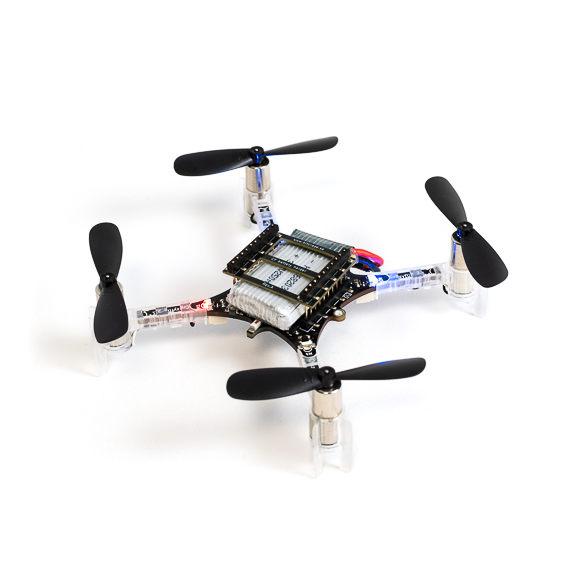
\includegraphics[width=0.5\textwidth]{figuras/crazyflie_2.1_585px.jpg}
    \caption{Crazyflie 2.1.}
    \cite{Crazyflie_2.1}
    \label{fig:Crazyflie 2.1}
\end{figure}

\subsection*{Control y estimación de estado}
La IMU del Crazyflie 2.1 cuenta con un acelerómetro/giroscopio de 3 de ejes BMI080 y un sensor de presión BMP388. El control del drone se basa en un modelo de sistema dinámico. El modelado de sistemas dinámicos es utilizado en sistemas de control y robótica para diseñar un controlador basado en la naturaleza del sistema, obteniendo un modelo matemático de este. Las variables de estado son valores determinados de un sistema dinámico, el cual puede ser un sistema físico, mecánico, eléctrico, etc. En el caso de un drone cuadricóptero, las variables de estado son los ángulos de rotación alrededor de sus ejes (\emph{roll}, \emph{pitch}, \emph{yaw}), su posición en el espacio y cómo estas variables cambian en el tiempo (sus derivadas). Para el caso de Crazyflie, las variables fundamentales a controlar son dichos ángulos y la altitud de este. Se utilizan estimaciones de estado para convertir las señales de los sensores en variables de estado y así poder realizar el respectivo control.  

Debido a que se utilizan métodos externos para determinar el estado de los drones, siendo un sistema de captura de movimiento para este caso, es necesario combinar las mediciones internas del drone con las externas por lo que se utiliza el filtro de Kalman como observador de estado. Los observadores de estado son algoritmos que utilizan el modelo matemático del sistema y mediciones del mismo para dar una estimación de las variables de estado. El filtro de Kalman es un observador de estado que toma en cuenta el ruido generado por perturbaciones en los actuadores o sensores del sistema, modelándolos como ruido blanco no correlacionado. Los drones Crazyflie utilizan un filtro de Kalman extendido como un filtro recursivo que estima el estado actual del drone basado en las mediciones internas y externas y el modelo matemático del mismo. \cite{Kalman}

El control de los drones se realiza mediante una arquitectura de controladores PID en cascada, donde la entrada de control es la posición y la velocidad esperada, que luego determina ángulos de \emph{pitch} y \emph{roll} deseados, seguido de una velocidad angular y finalmente determina el \emph{thrust} de los motores. \ref{fig:PID}
\begin{figure}[t]
    \centering
    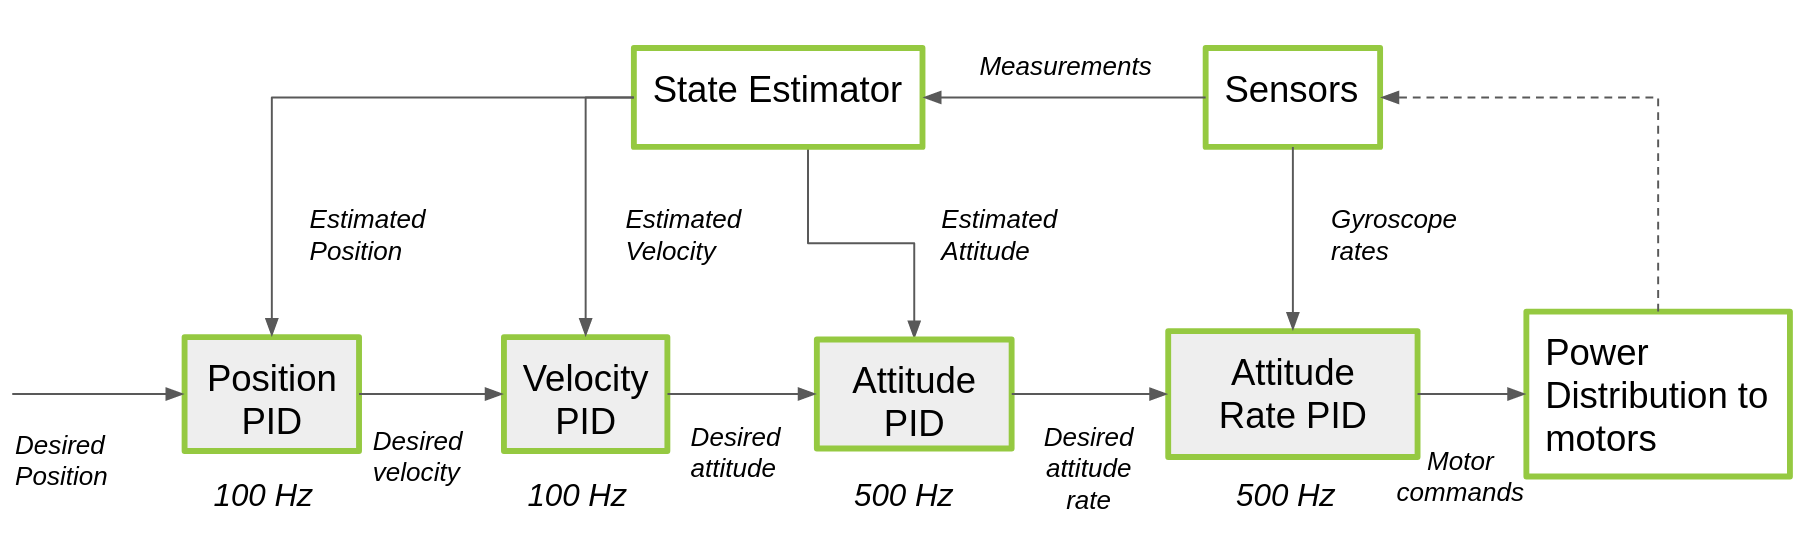
\includegraphics[width=0.8\textwidth]{figuras/cascaded_pid_controller.png}
    \caption{Arquitectura de Control.}
    \cite{Kalman}
    \label{fig:PID}
\end{figure}

\subsection*{Sistemas de radio frecuencia}
La comunicación por Radio Frecuencia (RF) es una tecnología para las telecomunicaciones que se da por un dispositivo que crea ondas electromagnéticas a altas frecuencias, donde las ondas se propagan en el espacio alcanzando a otro dispositivo receptor que procese la información a la misma frecuencia. Según la frecuencia de las ondas, las comunicación puede clasificarse en \begin{itemize}
    \item VLF: 3 kHz - 30 kHz
    \item LF: 30 kHz - 300 kHz
    \item HG: 3 MHz - 30 MHz
    \item VHF: 30 MHz - 300 MHz
    \item UHF: 300 MHz - 3 GHz
    \item SHF: 3 GHz - 30 GHz
    \item EHF: 30 GHz - 300 GHz
\end{itemize}
Las antenas convierten la información digital en señales eléctricas y luego en ondas electromagnéticas, o viceversa en el caso de la recepción de información. La ventaja que presenta este tipo de comunicación es que el dispositivo que procese tanto la información enviada como recibida puede ser un microcontrolador, siempre que este tenga la capacidad de conectarse a una antena y funcione a una frecuencia lo suficientemente alta como para procesar la señal de radio y digitalizar la información.

\subsection*{Protocolos de redes}
Para crear una comunicación eficiente se debe trabajar en conjunto con protocolos de comunicación por redes, como TCP, el cual divide la información en paquetes y garantiza que estos lleguen correctamente a su destino. El protocolo TCP, que significa \emph{Transmission Control Protocol}, es un protocolo de 3 vías donde primero se envía una solicitud inicial (\emph{SYN}) desde el origen, luego el destino envía un paquete de confirmación (\emph{SYN-ACK)} y finalmente el origen envía un último paquete (\emph{ACK}) seguido de la información a transmitir. Este trabaja en conjunto con el protocolo IP, el cual se encarga unicamente asegurar una conexión entre el servidor de origen y destino mediante el sistema de direcciones de Internet.

El \emph{User Datagram Protocol}, o UDP, es un protocolo de comunicación de Internet que, a diferencia del TCP, permite una comunicación rápida al no requerir que se establezca formalmente una conexión antes de iniciar con las transmisión de datos, sin embargo, esto también provoca que los paquetes puedan perderse en tránsito. \cite{UDP}

\subsection*{Formato JSON}
Para la estructura de los datos transferidos entre los distintos medios de comunicación, puede implementarse el formato \emph{JavaScript Object Notation} (JSON), el cual es ligero computacionalmente y de fácil lectura y escritura. Adicionalmente, puede aplicarse a otros lenguajes de programación, como C, C++, Python, etc.

\subsection*{Sistemas de captura de movimiento}

La captura de movimiento es una tecnología que ha ganado popularidad los últimos años al emplearse en aplicaciones como animación, videojuegos o investigación de sistemas mecánicos. Este proceso se da mediante cámaras de luz infrarroja, la cual se apunta hacia el sistema o conjunto de sistemas a capturar, los cuales deben contar con algún material que refleje la luz. En el caso particular de las cámaras de la marca Optitrack, las cuales son utilizadas en el Robotat en la Universidad del Valle de Guatemala (figura \ref{fig:camara}), cuentan con un set de emisores de luz infrarroja y utiliza pequeñas bolas cubiertas de material reflejante, conocidas como marcadores. Este tipo de captura de movimiento es conocido como óptica pasiva, ya que los marcadores reflejan la luz en lugar de generarla. \cite{Camilo2022_tesis}

\begin{figure}[t]
    \centering
    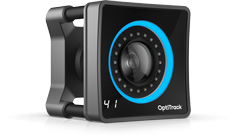
\includegraphics[width=0.5\textwidth]{figuras/primeX41-perspective-235.png}
    \caption{Cámara de captura OptiTrack.}
    \cite{OptiTrack_Primex-40}
    \label{fig:camara}
\end{figure}

Los marcadores pueden usarse de forma individual para rastrear unicamente posiciones, o bien pueden trabajarse en grupos de 3 con una forma en específico para analizar también la orientación de los cuerpos.

\subsection*{Ecosistema Robotat}

Para transferir los datos obtenidos por el sistema de captura en el Robotat, las cámaras OptiTrack están conectadas a un Switch que se comunica con un servidor mediante un protocolo UDP. La información es procesada  y enviada mediante un servidor de Python que posteriormente se comunica con un router Wi-Fi, el cual permite la comunicación entre dispositivos externos y agentes autónomos en el Robotat. Esta comunicación entre el router y los dispositivos se logra mediante un protocolo TCP, de esta forma puede accederse directamente a la información mediante la de composición de un documento de tipo JSON.

\subsection*{Cliente de Crazyflie y ROS2}

ROS funciona con nodos, creando un servidor de Crazyflie que establece la comunicación directa entre los drones y la interfaz utilizada, que en este caso es ROS2 junto con la API de Python como se ve en la Figura \ref{fig:nodos}.

El control de los drones se divide en cuatro capas independientes. La capa física transmite los paquetes de información desde y hacia el drone, donde puede implementarse una antena de radiofrecuencia para esto. El \emph{link} implementa los canales para los paquetes, abstrayendo el medio físico e implementando un canal de transmisión y otro de recepción entre el Crazyflie. El CRTP, acrónimo de \emph{Crazy Realtime Protocol}, implementa la información del puerto y el canal para crear la ruta del paquete a varios subsistemas. Finalmente, los subsistemas implementan las funcionalidades del Crazyflie que pueden ser controladas, habiendo sólo un puerto por subsistema.

\begin{figure}[t]
    \centering
    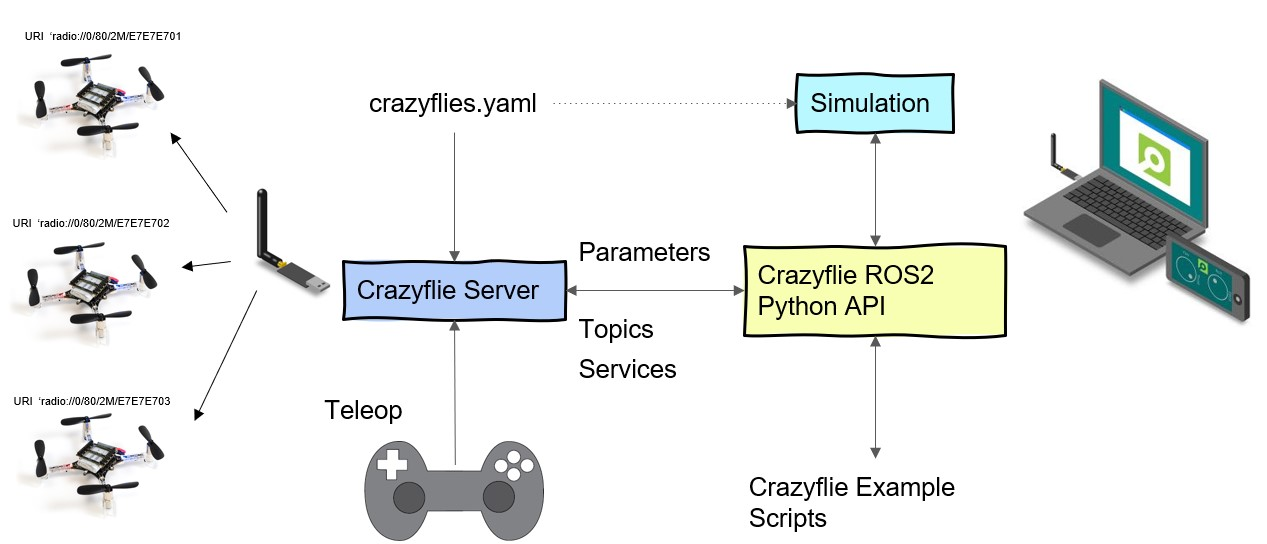
\includegraphics[width=0.5\textwidth]{figuras/overview_nodes.jpg}
    \caption{Estructura de control de Crazyswarm.}
    \cite{Crazyswarm2}
    \label{fig:nodos}
\end{figure}

El protocolo CRTP fue diseñado para permitir una priorización de paquetes y volver más eficiente la comunicación con el drone, permitiendo enviar una trayectoria mientras el drone se controla en tiempo real, siempre que el puerto de la trayectoria sea de mayor prioridad. Cada paquete CRTP contiene un puerto (4 bits), un canal (2 bits), y una carga de hasta 31 bytes. Para crear la conexión del protocolo se debe habilitar el \emph{link} USB usando un paquete de control USB, luego el \emph{link} Radio mantiene dos contadores de paquete para garantizar que no habrá pérdida de paquetes. Finalmente, el subsistema \emph{log} mantiene un estado de todos los bloques \emph{log} y continua enviado información aún si se pierde el \emph{link}\cite{CRTP}

Otro protocolo de comunicación para Crazyflie es el CPX (\emph{Crazyflie Packet eXchange}), el cual fue diseñado para funcionar a bajo nivel y que se empleen otros protocolos por encima. Su función es solucionar el problema de distribuir paquetes a través de múltiples microcontroladores ya que este problema no existía cuando se diseñó el protocolo CRTP, por lo que es un protocolo complementario. Debido a que se utiliza entre microcontroladores, puede enviarse de múltiples formas, como Wi-Fi/TCP, SPI o UART dependiendo de los microcontroladores a comunicar y los módulos adicionales que se implementen en el drone. Este protocolo permite el manejo de paquetes grandes, donde paquetes por debajo de 30 bytes se entregan en un bloque y paquetes más grandes pueden separarse en bloques y un identificador especifica cual es el bloque final.

Para establecer la comunicación de Crazyswarm, el servidor de Crazyflie se conecta con múltiples drones mediante una o más antenas de radiofrecuencia. Se cuenta con dos \emph{backends} a elegir, el ''cpp'' basado en la capa más baja y el ''cflib'', que funciona con Python a un nivel más alto. Este puede manejar aspectos de comunicación de bajo nivel, como recibir los parámetros del Crazyflie y convertirlos a parámetros de ROS2 para crear los parámetros de Crazyflie basado en la entrada.

Crazyflie cuenta con una máquina virtual, la cual funciona mediante Ubuntu y esta contiene todas las librerías para controlar los drones mediante una antena de radiofrecuencia USB. Estas librerías pueden visualizarse y editarse mediante Microsoft Visual Studio, que ya cuenta instalados los compiladores de C++ y Python. Desde Visual Studio, pueden iniciarse los códigos y, si la antena está conectada y un Crazyflie está encendido, pueden realizarse pruebas de movimiento y obtención de datos del drone. La máquina virtual también cuenta con el cliente de Crazyflie, desde el cual puede controlarse al Crazyflie mediante un control externo y es posible visualizar los ángulos de rotación del drone en tiempo real. En caso de que no se cuente con un control externo, puede utilizarse la aplicación para Android de Crazyflie y controlar al drone mediante \emph{Bluetooth}.

\begin{figure}[t]
    \centering
    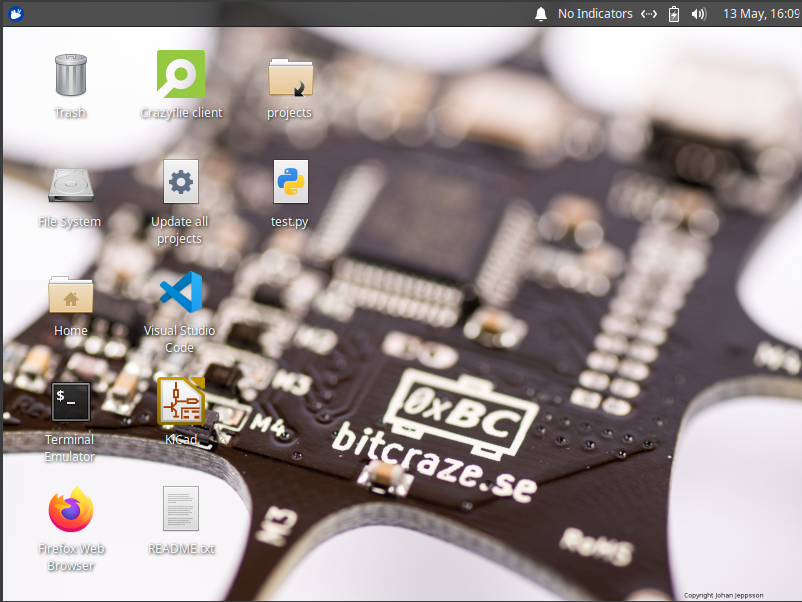
\includegraphics[width=0.5\textwidth]{figuras/VM_Crazyflie.png}
    \caption{Maquina Virtual de Crazyflie.}
    \label{fig:VM}
\end{figure}

Para poder realizar las pruebas del Crazyflie es necesario configurar el puerto de la antena durante la instalación de la máquina virtual, lo cual puede realizarse fácilmente mediante Oracle. También se deben configurar todos los dispositivos que se planeen utilizar en la máquina virtual, de lo contrario no serán reconocidos. Una vez instalada la máquina virtual se debe abrir una terminal e instalar ciertas librerías mediante el gestor de paquetes pip3. Las librerías son:
\begin{itemize}
    \item Matplotlib.
    \item Pandas.
    \item Canvas.
    \item pyinstaller.
\end{itemize}

Finalmente, es necesario actualizar las librerías de los controladores. Esto se logra mediante la opción incluída en el escrictorio de la máquina virtual, como se ve en la Figura 4 \ref{fig:VM}. Sin embargo, se presenta un problema al actualizar las librerías ya que luego de hacerlo deja de funcionar el cliente para controlar el drone con un control externo, por lo que si se desea trabajar con las librerías de Python y con el cliente se recomienda instalar dos máquinas virtuales y que una de estas no se actualice. 

